\graphicspath{%
{chapter5graph/}%
{chapter5graph/bg/}}
%\makeindex


\chapter{General}



\section{Confidence Interval}

\section{Conditional Probability}

Bayes's theorem is stated mathematically as the following equation:

\begin{eqnarray}
P(A|B) = \frac{P(B|A)P(A)}{P(B)}
\end{eqnarray}
where $A$ and $B$ are events and $P(B) \neq 0$.\\

P(A|B) is a conditional probability: the likelihood of event $A$ occurring given that $B$ is true. $P(A)$ and $P(B)$ are the probabilities of observing $A$ and $B$ respectively and they must be different event.\\

For conditional probability, $P(A|B)$ may or may not be equal to $P(A)$ (the unconditional probability of $A$). If $P(A|B) = P(A)$, then the events $A$ and $B$ are said to be independent. In this case, knowledge about either event does not alter the likelihood of each other. The definition (defined this way, not theoretical results) of the conditional probability is often quoted as :

\begin{eqnarray}
P(A|B) = \frac{P(A \cap B)}{P(B)}
\end{eqnarray}

This maybe visualised as restricting the sample space to situations in which $B$ occurs. The logic for this equation is that if the possible outcomes for $A$ and $B$ are restricted to those in which $B$ occurs, this set serves as the new sample space.

\begin{figure}[h!]
\begin{center}
	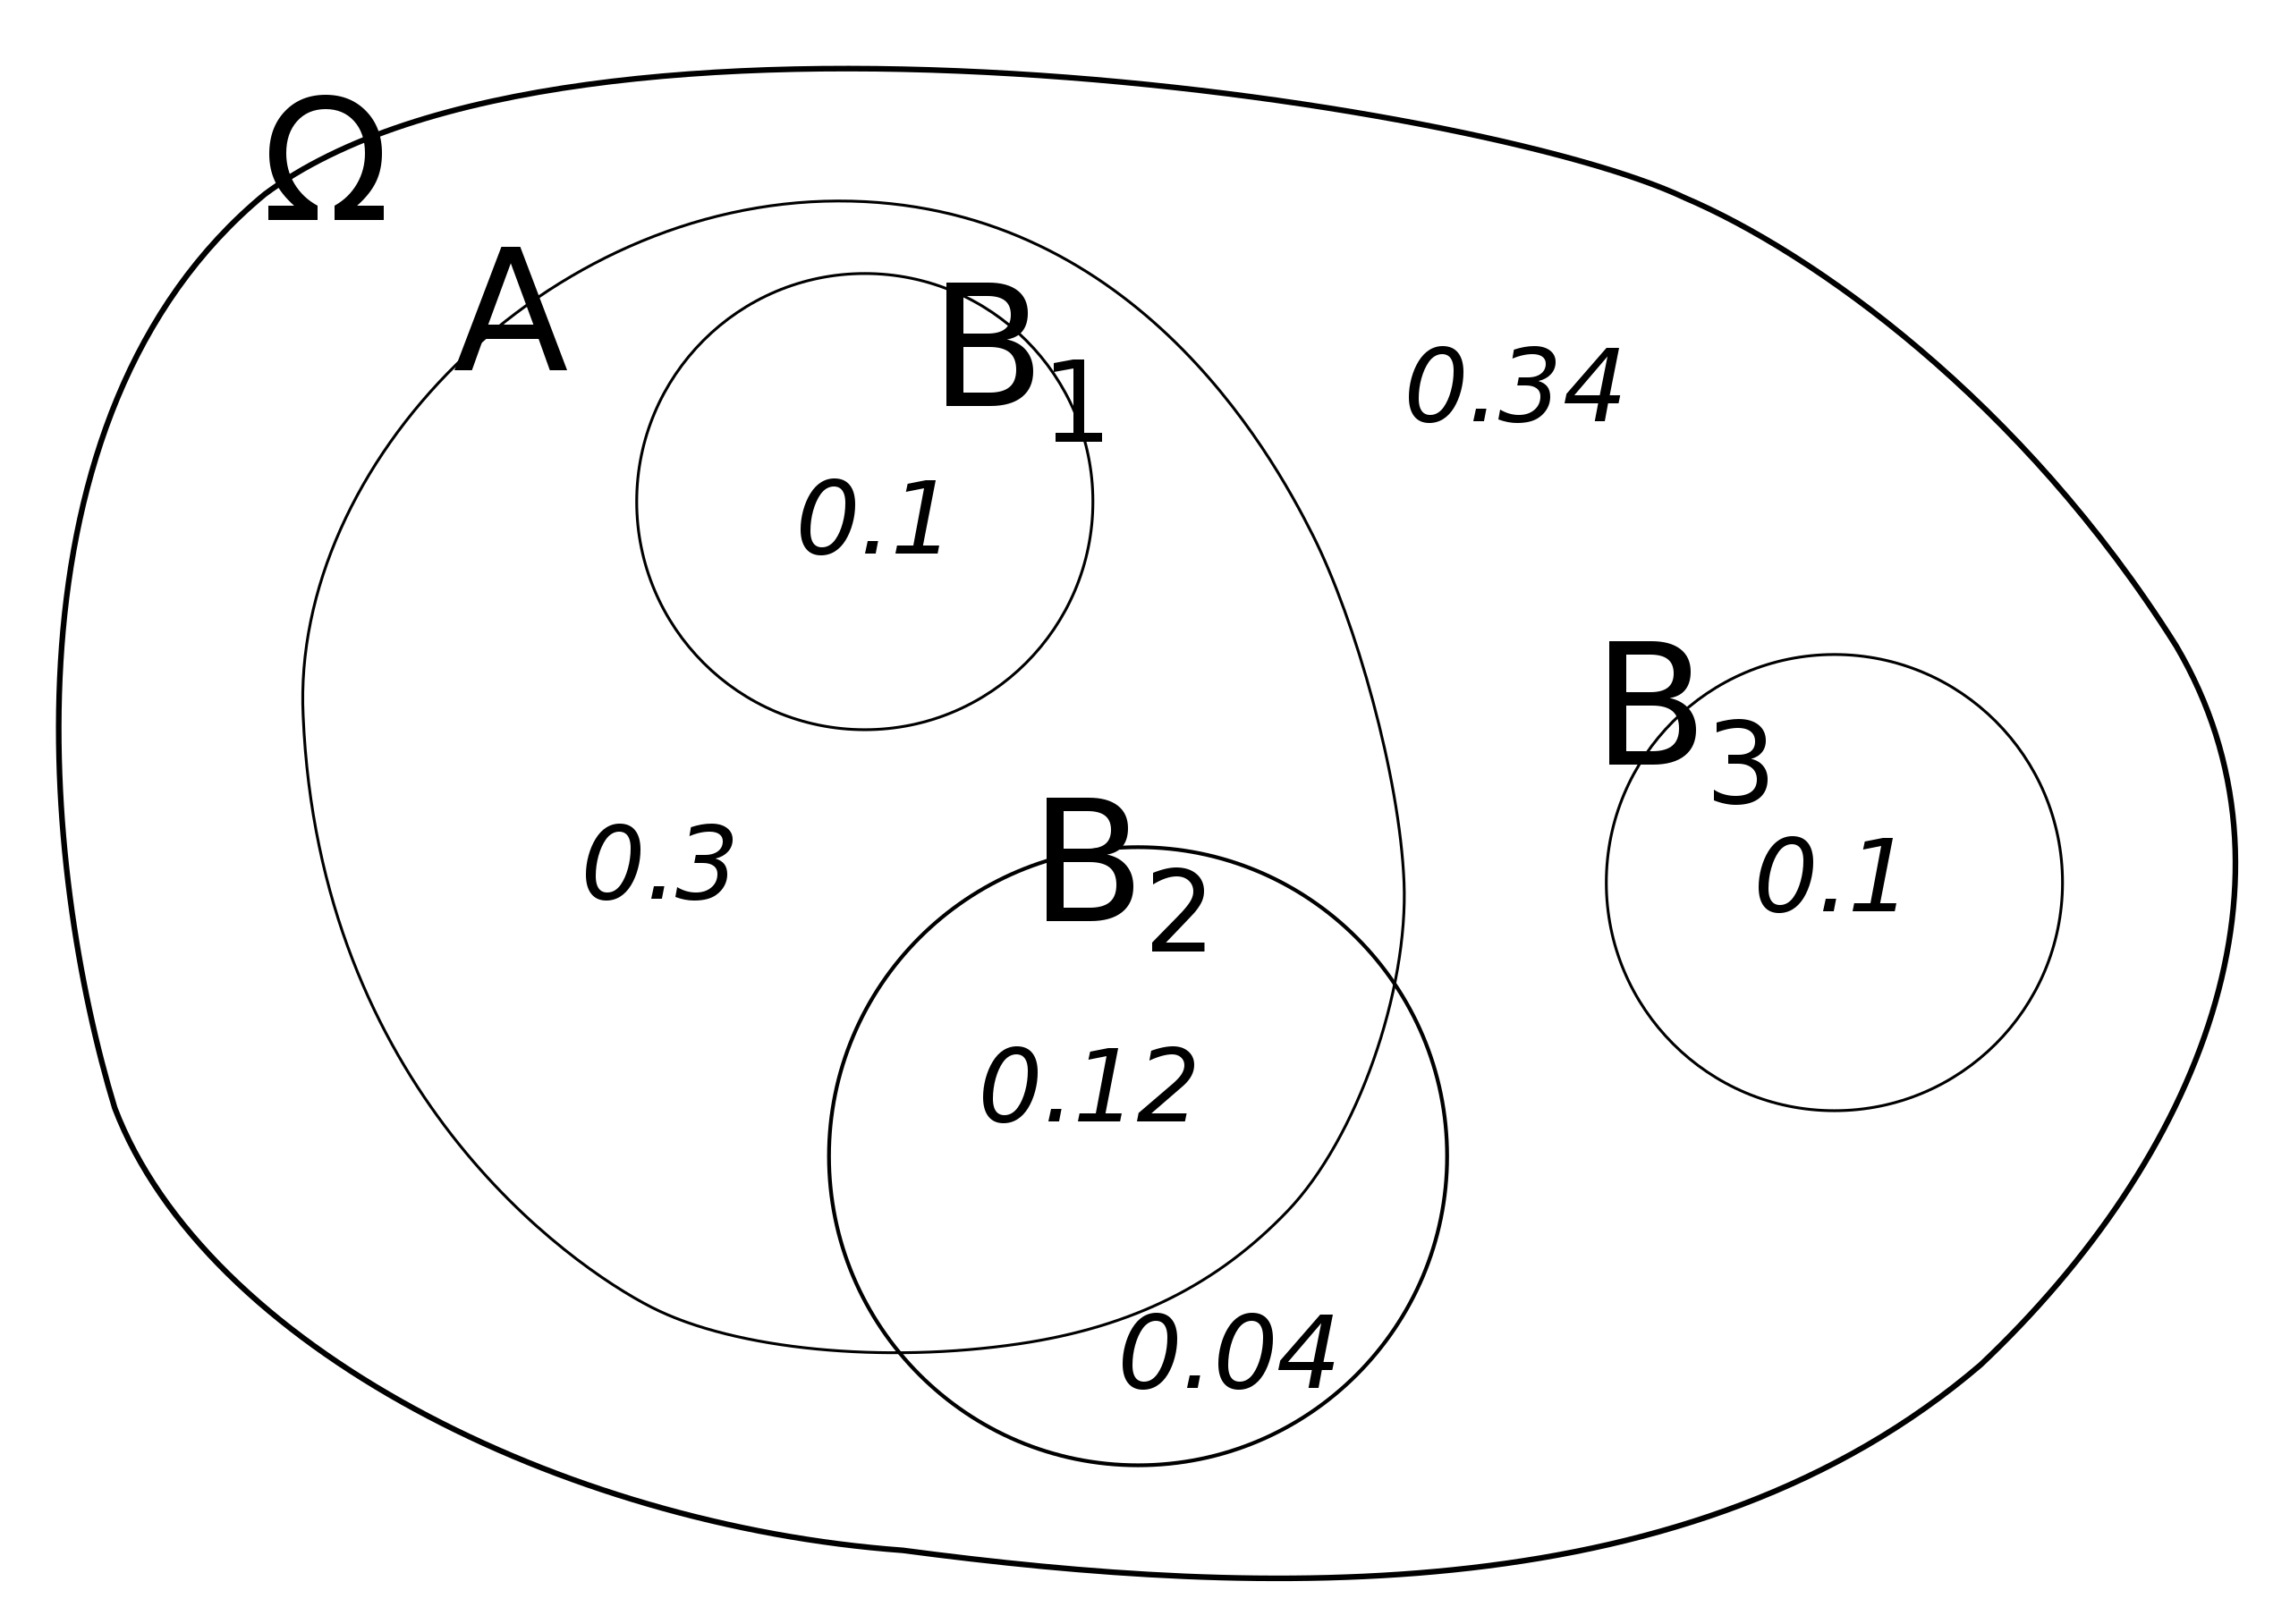
\includegraphics[scale=0.06]{condition_prob.png}
	\caption[]{Conditional probability with an Euler diagram}
	\label{condition_prob}
	\end{center}
	\end{figure}

The unconditional probability $P(A) = 0.3 + 0.1 + 0.12 = 0.52$. However, the conditional probability $P(A|B_1) = 1$, $P(A|B_2) = 0.12 / (0.12 + 0.04) = 0.75$, and $P(A|B_3) = 0$

\section{Normalisation}

\section{Standardisation}

\section{Least-squared error}

\section{R-squared error}

\section{Mean-squared error}

\section{Inferential Statistics}

\section{Bias-variance trade off}

The bias-variance tradeoff is the property of a model that the variance of the parameter estimates across samples can be reduced by increasing the bias in the estimated parameters. The bias-variance dilemma is the conflict in trying to simultaneously minimise these two sources of error that prevent supervised learning algorithm from generalising beyond their training set. \\\

The bias error is an error from erroneous assumptions in the learning algorithm. High bias can cause an algorithm to miss the relevant relations between features and target outputs, aka, underfitting. \\

The variance is an error from sensitivity to small fluctuations in the training set. High variance can cause an algorithm to model the random noise in the training data, rather than the intended outputs, aka, overfitting. \\

This trade-off is universal: it has been shown that a model that is asymptotically unbiased must have unbounded variance. \\

\begin{figure}[h!]
\begin{center}
	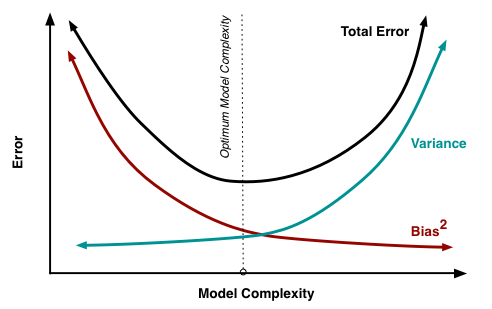
\includegraphics[scale=0.5]{b_v_tradeoff.png}
	\caption[]{Bias-variance trade-off.}
	\label{b_v_tradeoff}
	\end{center}
	\end{figure}

Dimensionality reduction and feature selection can decrease variance by simplifying models. Similarly, a larger training set tends to decrease variance. Adding features tends to decrease bias, at the expense of introducing additional variance. Learning algorithm typically have some tunable parameters that control bias and variations, some of the examples are:\\

1) Linear models can be regularised to decrease their variance at the cost of increasing their bias.\\
2) In neural network, variance increases and the bias decreases as number of hidden units hidden units increase. \\
3) In KNN, a high value of k leads to high bias and low variance. \\
4) In decision trees, the depth of the tree determines the variance. Decision trees are commonly pruned to control variance. (e.g. Reduced Error Pruning: starting at the leaves, each nodes is replaced with its most popular class, if the accuracy is not affected then the change is kept.) Pruning a node consists of removing all subtrees, making it a leaf, and assigning it the most common classification of the associated training examples. 







